\title{Master-Arbeit Exposee}
\author{
Konstantin Tkachuk
}
\date{\today}

\documentclass[12pt]{article}
\usepackage[utf8]{inputenc}
\usepackage[T1]{fontenc}
\usepackage{lmodern}
\usepackage[ngerman]{babel}
\usepackage{graphicx}


\begin{document}
\maketitle

\begin{abstract}
Dies ist ein kurzes Exposee für die geplante Master-Arbeit. Im ersten Teil werden die organisatorischen Aspekte der Arbeit angesprochen. Danach wird das Thema erläutert. Zum Schluss befindet sich eine erste Liste mit Literatur, die für die Arbeit relevant sein kann.
Es handelt sich hierbei um eine vorläufige Planung, Details können revidiert werden. 
\end{abstract}

\section{Organisatorisches}
\subsection{Bearbeiter}

Konstantin Tkachuk, konstantin.tkachuk@tu-dortmund.de, 0174/2496266

\subsection{Betreuer}
\begin{enumerate}
	\item Prof. Dr.-Ing. Olaf Spinczyk, OH 16, Raum E01, 0231/755-6322,\\
olaf.spinczyk@tu-dortmund.de
	\item Dr. Sven Seiler, Materna GmbH, 0231/5599-8902,\\ sven.seiler@materna.de
\end{enumerate}

\subsection{Zeitplanung}
Nachfolgend eine vorläufige Planung der zeitlichen Abfolge zur Masterarbeit. Die Zeiten können sich noch verschieben. Eine detaillierte Planung ist erst nach der Literaturrecherche und „state of the art“-Analyse möglich.
\begin{itemize}
	\item 15.06.2016: Start der Arbeit
	\item 30.06.2016: „State of the art“-Analyse abgeschlossen, Erster Architektur Entwurf
	\item 15.07.2016: Literaturrecherche und Inhaltsverzeichnis und Struktur der Arbeit beschlossen
	\item 15.07.2016: Anmeldung der Arbeit beim Prüfungsamt
	\item 15.08.2016: Fertigstellung eines Entwurf des Prototypen inkl. Datenmodell u. Systemarchitektur in UML
	\item 15.08.2016 – 15.11.2016: Implementierung
	\item 22.12.2016: Evaluation des Prototypen abgeschlossen
	\item 22.12.2016: „Draft“ der Arbeit fertig gestellt
	\item 15.01.2017: Arbeit fertig gestellt und Abgabe beim Prüfungsamt
\end{itemize}



\section{Inhaltliches}
\subsection{Arbeitstitel}
Vorläufiger Arbeitstitel, kann sich noch ändern. Evtl. ein äquivalenter Titel auf Deutsch:

\textbf{Open service and thing framework for smart reasoning based on Eclipse Open IoT Stack}


\subsection{Kurzbeschreibung des Themas}
Die enorm steigende Anzahl von „intelligenten Gegenständen“ mit eingebetteten Computern, die den Menschen im alltäglichen Leben unterstützen sollen, hat zu der Prägung des Begriffs „Internet der Dinge“ (IoT) geführt. Jedes dieser Dinge hat seine eigene Funktionalität und im Verbund stellen sie eine große Menge an Daten zur Verfügung. Gruppen von diesen Geräten sind bereits in übergreifende Services gebündelt, so können beispielsweise intelligente Leuchtmittel eines Herstellers durch eine von ihm bereitgestellte Schnittstelle über das Internet ferngesteuert werden. 

Thematisch eng verwoben mit IoT ist das Smart Home, welches die elektronische Steuerung von ausgewählten Geräten mit z.B. einer Rule Engine kombiniert um eine Automatisierung des Geräteverhaltens in einem Zusammenspiel zwischen Sensorik und Aktortik zu erreichen.
 
Leider befindet sich das systemübergreifende Zusammenspiel der unterschiedlichen Services derzeit noch in den Kinderschuhen. Services einzelner Hersteller sind proprietär und lassen sich nicht miteinander verknüpfen um ein Ganzes zu schaffen, was größer als die Summe seiner Teile wäre.

Aktuell gibt es zahlreiche Unternehmen und Frameworks, die sich mit den oben genannten Problemstellungen intensiv auseinandersetzen. Eine bekannte Lösung ist \textit{IFTTT}, welches eine große Anzahl verschiedener Services (\textit{Facebook}, \textit{Philips Hue}, \textit{Dropbox}, etc.) integriert und eine rudimentäre Rule Engine anbietet, die es erlaubt auf eine einfache Art und Weise serviceübergreifende „if this than that“ Anweisungen zu hinterlegen, die der klassischen „EDV“ ähneln. Bis dato lassen sich komplexere Szenarien mit \textit{IFTTT} nicht abbilden. 

Von anderen Anbietern werden für IoT ausgelegte Rule Engines verschiedener Komplexität angeboten. Hierzu gehören beispielsweise die Rule Engine des AWS IoT, welche speziell auf die Zusammenarbeit der verschiedenen Amazon Web Services ausgelegt ist oder die \textit{Waylay} Rule Engine, die komplexe Inferenzen und den Umgang mit Unsicherheit anbietet.

Ziel dieser Arbeit ist es ein über die o.g. Ansätze hinausgehendes Framework zu schaffen, welches als zentrale Schnittstelle für die Zusammenarbeit und zum Mediieren von sowohl Services als auch Dingen dienen soll. Es soll offen sein für die Einbindung von neuen Entitäten. Bei den Services kann es sich sowohl um Gerätesteuerungsdienste, wie \textit{Garage.IO} oder \textit{Philips Hue}, als auch hardwareunabhängige Dienste wie die \textit{Flickr API} oder \textit{Twitter} handeln. Gleichzeitig soll das Framework in der Lage sein Dinge direkt anzusteuern.

Außerdem soll das Framework es ermöglichen das Verhalten von Services und Dingen zu automatisieren. Dabei sollen verschiedene Entitäten miteinander interagieren und durch das Framework mediiert werden können. Beispielsweise können in einem Smart Home nahen Szenario bei Öffnen der Garagentür die Lichter im Haus angehen. Dabei würden die Information, dass die Garagentür geöffnet wurde, durch den \textit{Garage.IO} Service bereitgestellt und die Lampen durch \textit{Philips Hue} (oder direkt, wenn z.B. das Framework lokal installiert ist) gesteuert werden. Alternativ sind auch Smart Home ferne Szenarien möglich, wie das automatische Posten eines Tweets wenn ein Foto gemacht wurde. 

Das Framework soll basierend auf dem \textit{Eclipse Open IoT Stack} (siehe Abbildung \ref{fig:eclipse}) entwickelt werden. Der \textit{Eclipse Open IoT Stack} ist eine Sammlung von mehreren Frameworks die auf Java OSGi basieren. \textit{Eclipse Paho}, \textit{Eclipse Californium} und \textit{Eclipse Wakaama} unterstützen die Verbindungsprotokolle MQTT, CoAP und LWM2M respektive. \textit{Eclipse Kura} bietet unterstützende Dienste für IoT Gateways. Hierzu gehören u.a. I/O-, Data-, Cloud-, Configuration und andere Services. \textit{Eclipse SmartHome}, \textit{Eclipse SCADA} und \textit{Eclipse OM2M} runden den Open IoT Stack ab, indem sie Unterstützung für Hausautomatisierung, SCADA Systeme und Telco Dienste anbieten.

\begin{figure}[h]
    \centering
    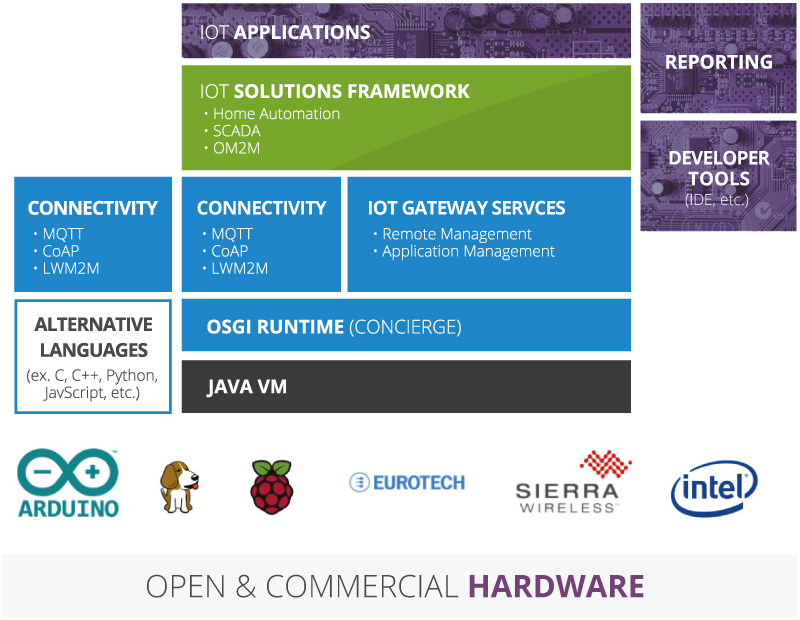
\includegraphics[width=\textwidth]{eclipse}
    \caption{Eclipse Open IoT Stack Struktur}
    \label{fig:eclipse}
\end{figure}

Im Rahmen der Arbeit soll geprüft werden, in welchem Maße die von Eclipse SmartHome bereitgestellten Funktionalitäten für einen Einsatz im übergeordneten IoT Umfeld geeignet sind. Gegebenenfalls sollen diese Funktionalitäten im zu entwickelnden Framework aufgegriffen und um notwendige weitere Features erweitert werden, sodass die Offenheit gegenüber der Integration und intelligenter Interaktion mit anderen Arten von Services (z.B. Social Media, File Sharing, etc.) gewährleistet wird. 
%TLDR: smarthome erweitern, sodass mit services umgangen werden kann

Aus einer wissenschaftlichen Perspektive befindet sich das Internet der Dinge gerade auf dem Gipfel der überzogenen Erwartungen (siehe Abbildung \ref{fig:hype}). Bevor das „Plateau der Produktivität“ jedoch erreicht wird, muss noch viel geforscht werden. Es gibt Fragen zu beantworten, welche die Themen Architektur und Abhängigkeiten, Big Data, Robustheit, Offenheit, Sicherheit und weitere betreffen. Auch das Problem der mangelnden Standardisierung wird immer wieder aufgegriffen.

\begin{figure}
    \centering
    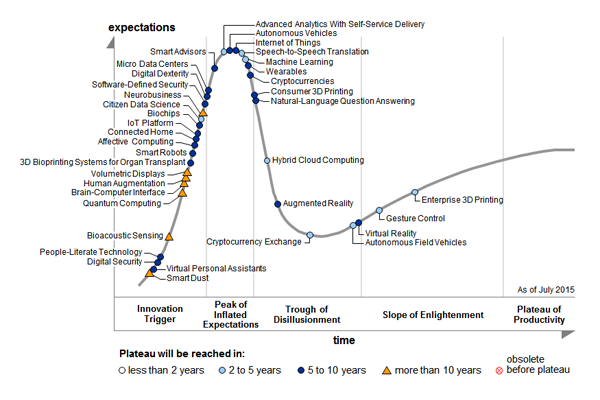
\includegraphics[width=\textwidth]{hype}
    \caption{Hype Cycle (http://www.gartner.com/newsroom/id/3114217)}
    \label{fig:hype}
\end{figure}

Das \textit{European Research Cluster on the Internet of Things} (IERC) forscht seit Jahren im Rahmen des \textit{7th Framework Programme} an aktuellen IoT Themen im Rahmen zahlreicher Forschungsprojekte. Es werden z.B. Versuche unternommen, unterschiedliche Technologien (Cloud Computing, Machine-2-Machine Learning und andere) mit IoT zu kombinieren und die Ergebnisse evaluiert.

Aktuell sind Frameworks stets auf jeweils einen konkreten Bereich des IoT spezialisiert. Smart Home Frameworks beschäftigen sich mit der direkten Steuerung von Dingen. \textit{IFTTT} arbeitet auf einer höheren Abstraktionsebene, indem es nur mit Services interagiert, ohne in direkten Kontakt mit Dingen zu kommen. Bisher existieren jedoch keine Lösungen, die diese Funktionalitäten in einem gemeinsamen Kontext anbieten. An dieser Stelle soll die Arbeit ansetzen. Dabei soll auf den Ergebnissen aktueller Forschung in Bereichen IoT Architektur, Service Orchestration, Cloud Computing und anderen aufgebaut werden.










\bibliographystyle{abbrv}
\nocite{*}
\bibliography{Expose}

\end{document}

